\documentclass[presentation.tex]{subfiles} 

\begin{document}

\begin{frame}
	\frametitle{Porovnanie $L^1$ a $L^{\infty}$ lineárnej regresie}
	
	\begin{itemize}
		\item $L^1$ -- veľmi dobre zachytáva lineárny vzťah, môže viesť k \textit{overfittingu}
		\item $L^{\infty}$ -- príliš ovplyňovaná outliermi
	\end{itemize}
	
	\begin{columns}
		\begin{column}{0.5\textwidth}
			\centering
			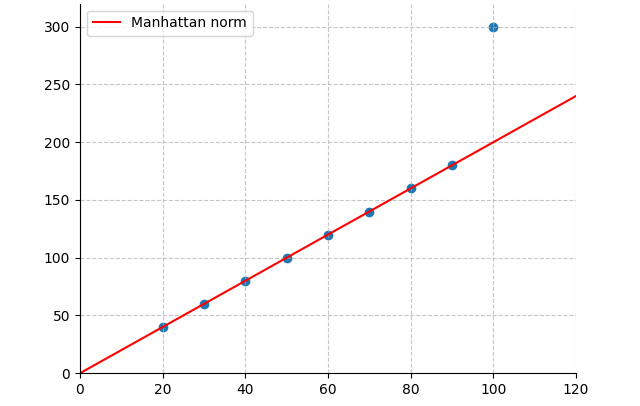
\includegraphics[width=\linewidth]{../report/figs/L1_linear_with_outlier_cropped.png}
			\captionof*{figure}{regresia $L^1$ normou}
		\end{column}
		\begin{column}{0.5\textwidth}
			\centering
			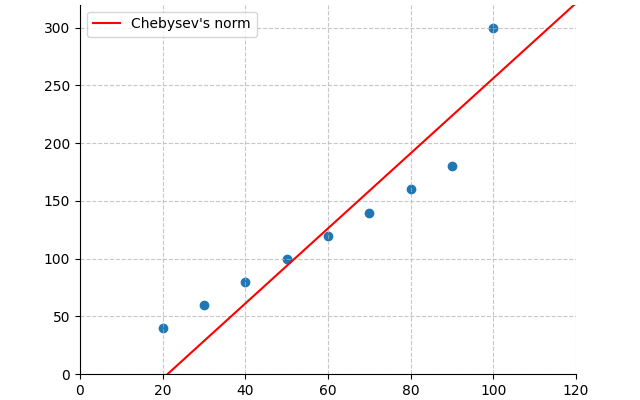
\includegraphics[width=\linewidth]{../report/figs/LInf_linear_with_outlier_cropped.png}
			\captionof*{figure}{regresia $L^{\infty}$ normou}
		\end{column}
	\end{columns}
	
\end{frame}


\begin{frame}
	\frametitle{Minimalizácia váženého súčtu noriem}
	
	\begin{itemize}
		\item redukcia \textit{overfittingu} $L^1$ regresie váženým súčtom s $L^{\infty}$ normou
	\end{itemize}
	\begin{equation*}
		\min ~ \omega||y - \hat{y}||_1 + (1-\omega)||y - \hat{y}||_{\infty},~\omega \in [0;1]
	\end{equation*}
	\vspace{-0.8cm}
	\begin{itemize}
		\item stále implementovateľné ako úloha lineárneho programovania
	\end{itemize}
{\scriptsize
	\setlength{\abovedisplayskip}{6pt}
	\setlength{\belowdisplayskip}{\abovedisplayskip}
	\setlength{\abovedisplayshortskip}{0pt}
	\setlength{\belowdisplayshortskip}{3pt}
\begin{align*}
	\text{min}~ &
	\left(
	\begin{array}{c|c|c}
		\mathbf{0}_{k+1}^T ~ & ~\omega\mathbf{1}_n^T ~& ~(1 - \omega)
	\end{array}
	\right)
	\left(
	\begin{array}{c}
		\beta \\
		\hline
		t \\
		\hline
		\gamma
	\end{array}
	\right), ~ \omega \in [0; 1]\\
	&\left(
	\begin{array}{c|c|c}
		\mathbf{A} ~&~ \mathbb{I}_n ~&~ \mathbf{0}_n \\
		\hline
		-\mathbf{A} ~&~ \mathbb{I}_n ~&~ \mathbf{0}_n \\
		\hline
		\mathbf{A} ~&~ \mathbf{0}_{n \times n} ~&~ \mathbf{1}_n \\
		\hline
		-\mathbf{A} ~&~ \mathbf{0}_{n \times n} ~&~ \mathbf{1}_n \\
	\end{array}
	\right)
	\left(
	\begin{array}{c}
		\beta \\
		\hline
		t \\
		\hline
		\gamma
	\end{array}
	\right)
	\geq
	\left(
	\begin{array}{c}
		y \\
		\hline
		-y \\
		\hline
		y \\
		\hline
		-y
	\end{array}
	\right) \\
	&\beta \in \mathbb{R}^{k+1},~t \geq \mathbf{0}_{n},~\gamma \geq 0
\end{align*}
}%
\end{frame}

\begin{frame}
	\frametitle{Minimalizácia váženého súčtu noriem}
	\begin{itemize}
		\item implementované ako \pyth|WeightedL1LInfModel|
	\end{itemize}
	\begin{columns}
		\begin{column}{0.5\textwidth}
			\centering
			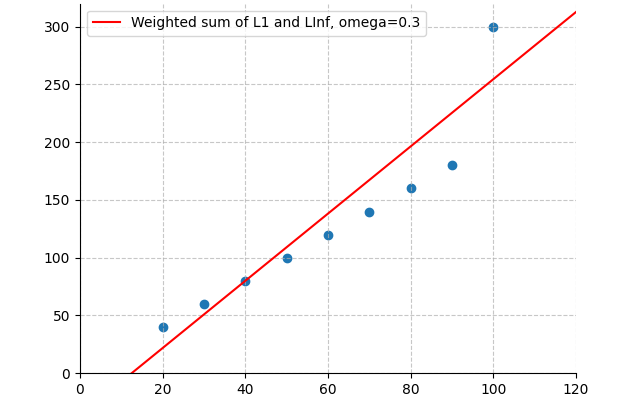
\includegraphics[width=\linewidth]{../report/figs/weighted_linear_with_outlier_cropped.png}
			\captionof*{figure}{regresia váženým súčtom noriem}
		\end{column}
		\begin{column}{0.5\textwidth}
			\centering
			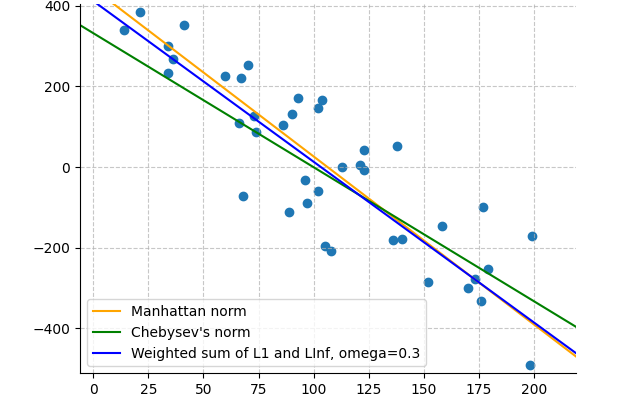
\includegraphics[width=\linewidth]{../report/figs/all_three_random_cropped.png}
			\captionof*{figure}{porovnanie troch regresií}
		\end{column}
	\end{columns}
	
\end{frame}
	
\end{document}